\subsection*{Zadania: Reakcje podporowe}

Wyznacz reakcje podporowe w poniższych przykładach. Uwzględnij ciężar własny tarczy tam, gdzie podany jest ciężar powierzchniowy. W pozostałych przypadkach pomiń go.

\begin{figure}[htbp]
    \centering
    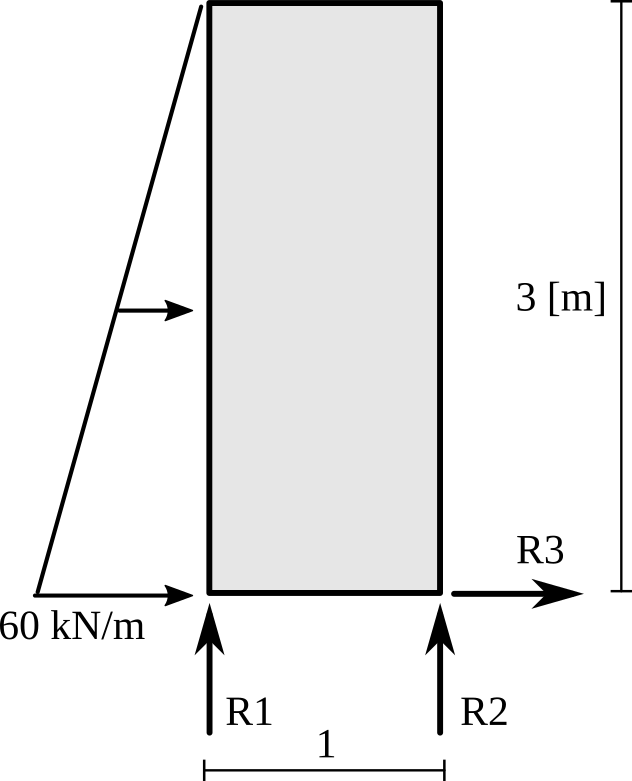
\includegraphics{Reakcje/Tarcza01.png}
    \caption{Układ A - obciążenie rozłożone trójkątne}
\end{figure}

\begin{figure}[htbp]
    \centering
    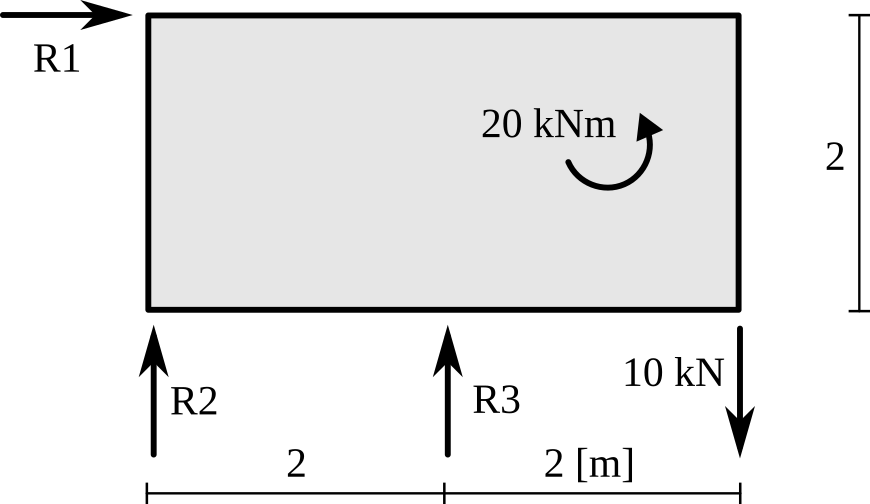
\includegraphics{Reakcje/Tarcza02.png}
    \caption{Układ B - siły i momenty skupione}
\end{figure}

\begin{figure}[htbp]
    \centering
    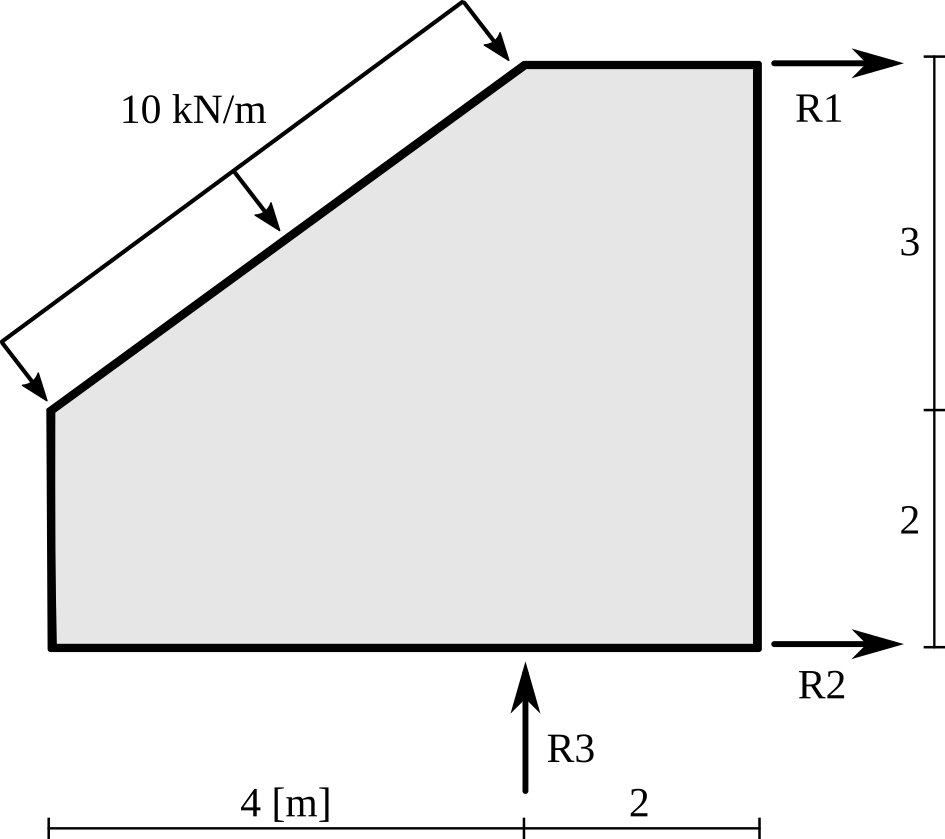
\includegraphics{Reakcje/Tarcza03.png}
    \caption{Układ C - obciążenie rozłożone na odcinku ukośnym}
\end{figure}

\begin{figure}[htbp]
    \centering
    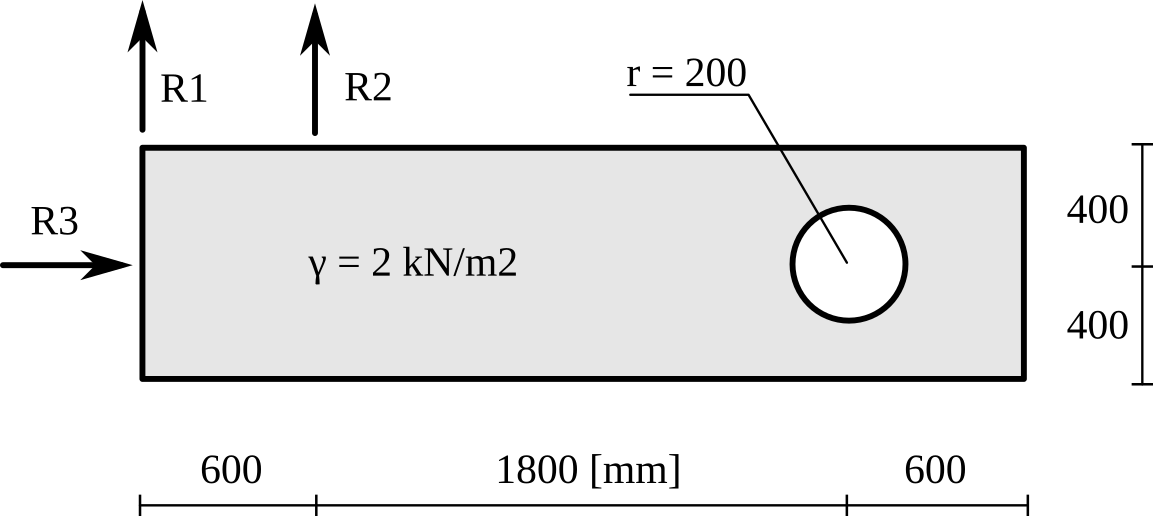
\includegraphics{Reakcje/Tarcza04.png}
    \caption{Układ D - ciężar własny}
\end{figure}